\documentclass[12pt, aspectration=169]{beamer}
\usetheme{CambridgeUS}
\usecolortheme{seahorse}
\setbeamertemplate{navigation symbols}{}
\usepackage[utf8]{inputenc}
\usepackage{graphicx}
\usepackage{multicol}
\usepackage{hyperref}

\setbeamertemplate{frametitle continuation}[from second]

\title{Progetto di ingegneria del software, Team3}
\author{Juan Guillermo Jaramillo Saa (SM) \\
        Daniele Tarek Iasy (PO) \\ 
        Alexandru Bogdan Nicolescu (DEV) \\ 
        Andrea Largura (DEV) \\
        Riccardo Fava (DEV)}
\institute[]{Universit\'a di Bologna, Corso di Laurea in Informatica}
\date{14 Dicembre 2022}

\begin{document}
\maketitle
\begin{frame}{Sommario}
\begin{itemize}
    \item Descrizione del prodotto
    \item Backlog di prodotto
    \item Sprint 1
    \item Sprint 2
    \item Sprint 3
    \item Sprint 4
    \item Conclusioni
\end{itemize}
\end{frame}
\begin{frame}{Prodotto}
\framesubtitle{Descrizione del prodotto.}
Si \`e sviluppato un client di twitter in grado di: 
\begin{itemize}
    \item Effettuare ricerche, filtrandone i risultati
    \item Visualizzare statistiche su tali ricerche
    \item Giocare agli scacchi, tramite il meccanismo delle risposte dei tweet
    \item Ottenere informazioni interessanti sulla ghigliottina e sul fantacitorio
\end{itemize}
\end{frame}
\begin{frame}{Prodotto}
\framesubtitle{Backlog di prodotto.}
\begin{multicols}{2}
Ricerche:
\begin{itemize}
\item \`E possibile cercare tweet con specifiche parole, quali:
\begin{itemize}
    \item parole chiave
    \item hashtag
    \item menzioni di utenti specifici (tramite @)
\end{itemize}
\item Tweet di un utente
\item Stream di hashtag
\end{itemize}
\columnbreak

Filtri:
\begin{itemize}
\item Intervalli di date (dell'ultima settimana e non)
\item Numero di risultati
\end{itemize}
Scacchi:
\begin{itemize}
    \item Partita tramite sfidanti nelle risposte del tweet della partita
\end{itemize}
\end{multicols}
\end{frame}
\begin{frame}{Prodotto}
\framesubtitle{Backlog di prodotto. (Cont.)}
\begin{multicols}{2}
Visualizzazaioni:
\begin{itemize}
\item Wordcloud della ricerca
\item Sentiment della ricerca / dei singoli tweets
\item Distribuzione temporale dei tweet
\item Visualizzazione su mappa
\end{itemize}

\columnbreak
Giochi televisivi:
\begin{itemize}
\item Fantacitorio
\begin{itemize}
    \item Classifica settimanale / di sempre dei politici
    \item Squadre della settimana, o di un utente
\end{itemize}
\item Eredit\'a
\begin{itemize}
    \item Parole vincenti della settimana
    \item Username dei campioni
\end{itemize}
\end{itemize}
\end{multicols}
\end{frame}
\begin{frame}{Sprint 1, 19 Ottobre - 2 Novembre}
\framesubtitle{Sprint goal \& \href{https://taiga.hjkl.gq/project/ingsw2022-team3/taskboard/sprint-1-5}{backlog}}
Il nostro obiettivo fin da questo sprint è stato quello di portare un client che potesse effettuare ricerche di tweet per parola chiave. \\
Backlog:
\begin{itemize}
    \item ricerca di tweet per specifiche parole (8 punti)
    \item homepage del sito (13 punti)
\end{itemize}
\end{frame}
\begin{frame}{Sprint 1, 19 Ottobre - 2 Novembre}
\framesubtitle{Lo sprint}
Questo \`e stato uno sprint in cui ci siamo concentrati sul team e sulle principali scelte progettuali per la realizzazione del prodotto: un'applicazione web con frontend in React e backend in Node + Express. \\
Inoltre siamo riusciti a portare una buona demo il sprint review
\end{frame}
\begin{frame}{Sprint 1, 19 Ottobre - 2 Novembre}
\framesubtitle{\href{https://taiga.hjkl.gq/project/ingsw2022-team3/wiki/sprint-rw-3110}{Lo stato di avanzamento}}
\begin{figure}[H]
    \centering
    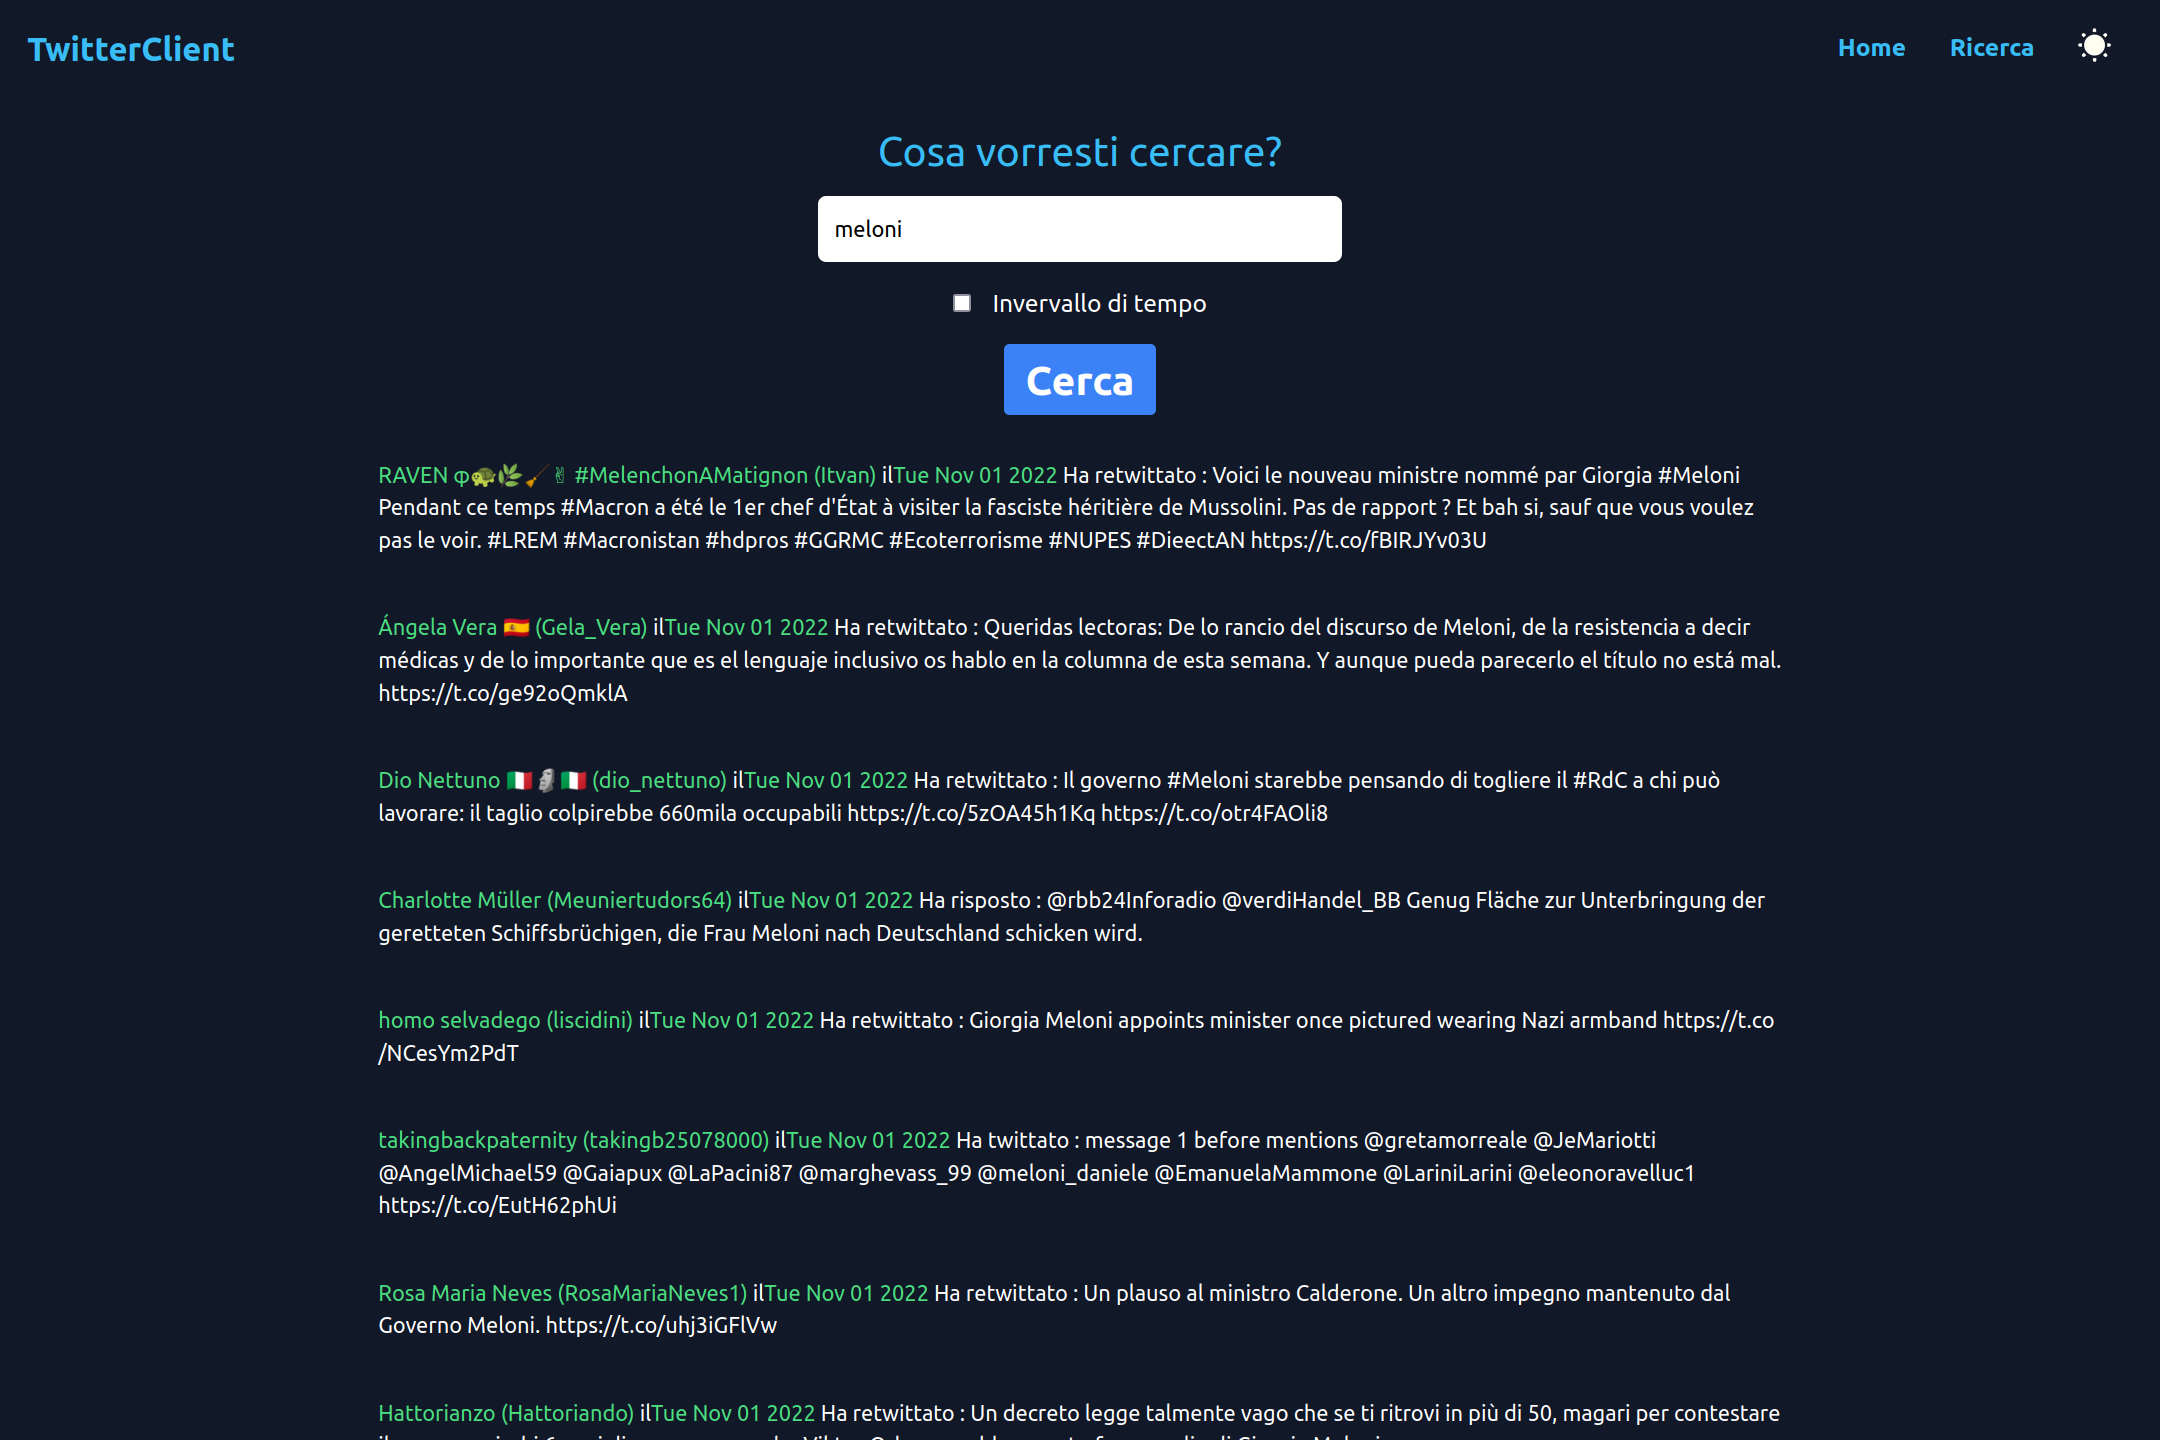
\includegraphics[scale=0.15]{reviews/sprint_review1031.png}
    \label{fig:review1}
\end{figure}
\end{frame}
\begin{frame}{Sprint 1, 19 Ottobre - 2 Novembre}
\framesubtitle{\href{https://taiga.hjkl.gq/project/ingsw2022-team3/wiki/retrospettiva-sprint-1}{Retrospettiva}}
Dalla retrospettiva sono sorte diverse problematiche, tra cui:
\begin{itemize}
    \item Non abbiamo esplicitato una DOD e lo sprint goal
    \item Niente test
\end{itemize}
\href{https://taiga.hjkl.gq/project/ingsw2022-team3/wiki/retrospettiva-sprint-1}{Restrospettiva su taiga}
\end{frame}
\begin{frame}{Sprint 2, 2 Novembre - 16 Novembre}
\framesubtitle{Sprint goal \& \href{https://taiga.hjkl.gq/project/ingsw2022-team3/taskboard/sprint-2-5}{backlog}}
Il goal \`e stato portare alla demo un client che permettesse di filtrare ricerche e visualizzare statistiche di sentiment analysis e di distribuzione temporale su tali ricerche. \\
Backlog:
\begin{itemize}
    \item ricerca di tweet di un utente (15 punti)
    \item filtro di intervallo di date (14 punti)
    \item filtro di numero di risultati (15 punti)
    \item statistiche di sentiment analysis (28 punti)
    \item visualizzazione mappa (13 punti)
    \item visualizzazione distribuzione temporale (13 punti)
\end{itemize}
\end{frame}
\begin{frame}{Sprint 2, 2 Novembre - 16 Novembre}
\framesubtitle{Lo sprint}
Questo sprint \`e stato impegnativo, abbiamo scelto tante funzionalit\'a da implementare, inoltre abbiamo dato il via ai test (solo del backend).
\end{frame}
\begin{frame}{Sprint 2, 2 Novembre, 16 Novembre}
\framesubtitle{\href{https://taiga.hjkl.gq/project/ingsw2022-team3/wiki/sprint-rw-1511}{Lo stato di avanzamento}}
\begin{figure}[H]
    \centering
    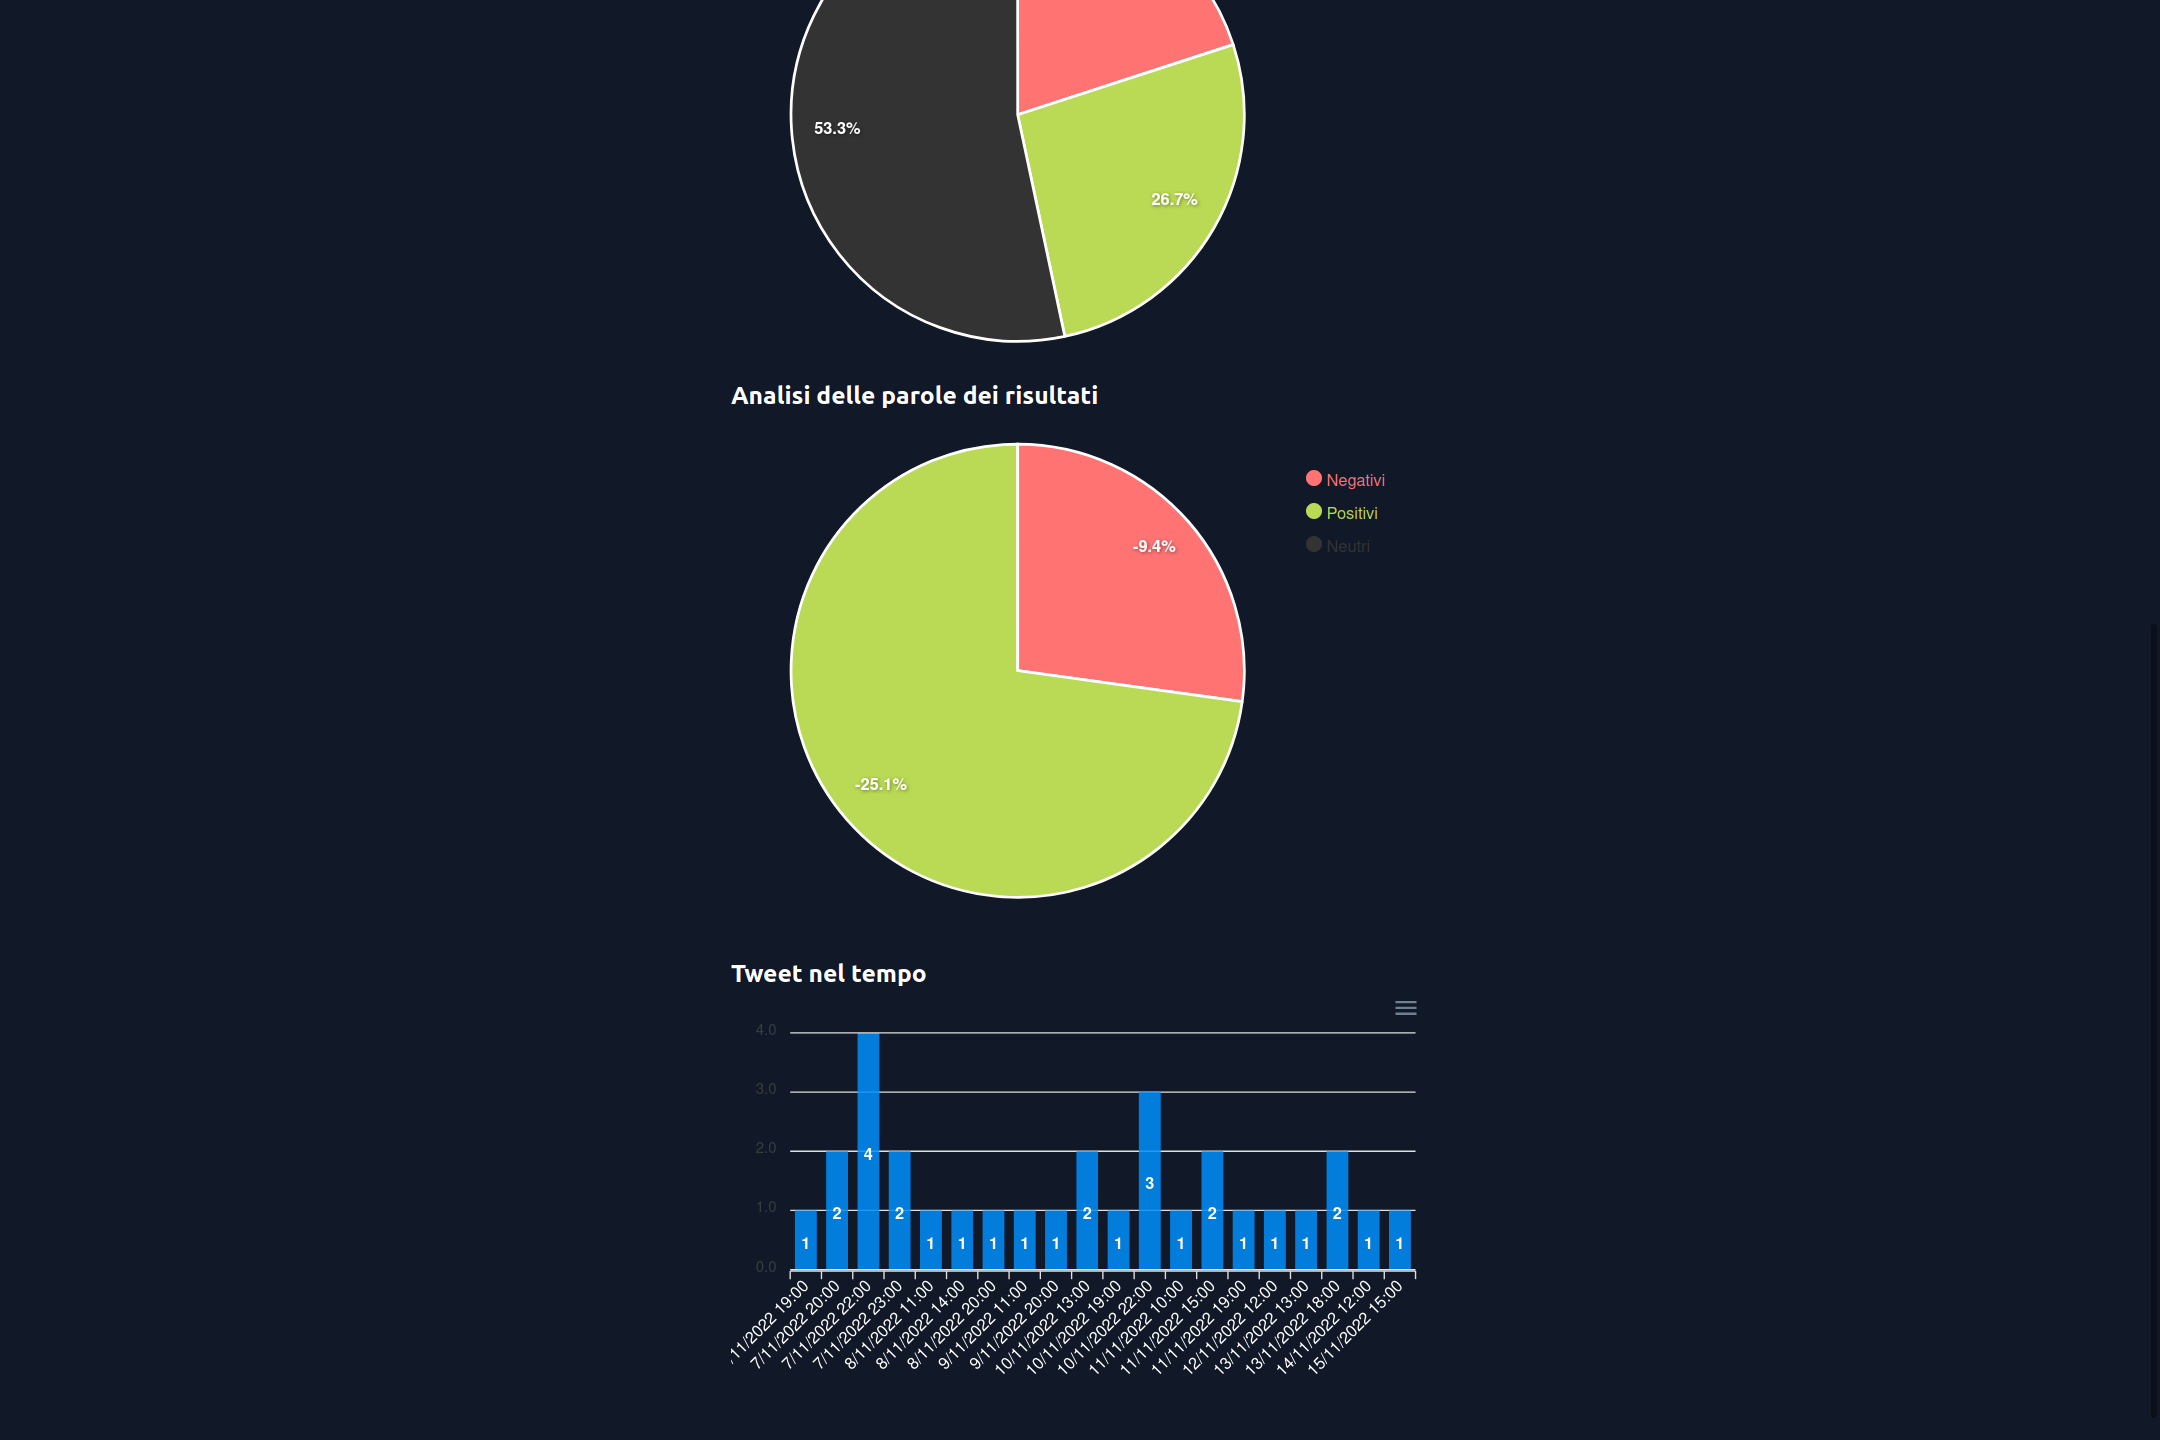
\includegraphics[scale=0.15]{reviews/sprint_review1115.png}
    \label{fig:review2}
\end{figure}
\end{frame}
\begin{frame}{Sprint 2, 2 Novembre - 16 Novembre}
\framesubtitle{\href{https://taiga.hjkl.gq/project/ingsw2022-team3/wiki/retrospettiva-sprint-2}{Retrospettiva}}
Lo sprint \`e andato molto bene rispetto a quello precedente, le criticit\'a che erano emerse, sono state superate. \\
In generale, tra le cose che sarebbero potute andare meglio, vi \`e la DOD, infatti non abbiamo incluso i test automatici del codice perch\'e non sapevamo quanto sarebbe stato impegnativo documentarsi sui framework e/o librerie di testing. \\
\href{https://taiga.hjkl.gq/project/ingsw2022-team3/wiki/retrospettiva-sprint-2}{Retrospettiva su taiga}
\end{frame}
\begin{frame}{Sprint 3, 16 Novembre - 30 Novembre}
\framesubtitle{Sprint goal \& \href{https://taiga.hjkl.gq/project/ingsw2022-team3/taskboard/sprint-3-6}{backlog}}
Il goal \`e stato quello di portare un client che permettesse di effettuare statistiche utili, interessanti sulle ricerche effettuate oltre al permettere di visualizzare i campioni della ghigliottina su twitter. \\
Backlog:
\begin{itemize}
    \item visualizzazione della wordcloud della ricerca (15 punti)
    \item la ghigliottina (32 punti)
    \begin{itemize}
        \item parole vincenti della settimana
        \item campioni della settimana
    \end{itemize}
\end{itemize}
\end{frame}
\begin{frame}{Sprint 3, 16 Novembre - 30 Novembre}
\framesubtitle{Lo sprint}
In questo sprint ci siamo concentrati sul risolvere gli issue (e.g. \href{https://taiga.hjkl.gq/project/ingsw2022-team3/issue/94}{sentimenti singoli dei tweet}) che erano stati sollevati dal professore durante la sprint review dello scorso sprint, inoltre abbiamo iniziato ad adottare pratiche di CI.
\end{frame}
\begin{frame}{Sprint 3, 16 Novembre - 30 Novembre}
\framesubtitle{\href{https://taiga.hjkl.gq/project/ingsw2022-team3/wiki/sprint-rw-512}{Lo stato di avanzamento}}
\begin{figure}[H]
    \centering
    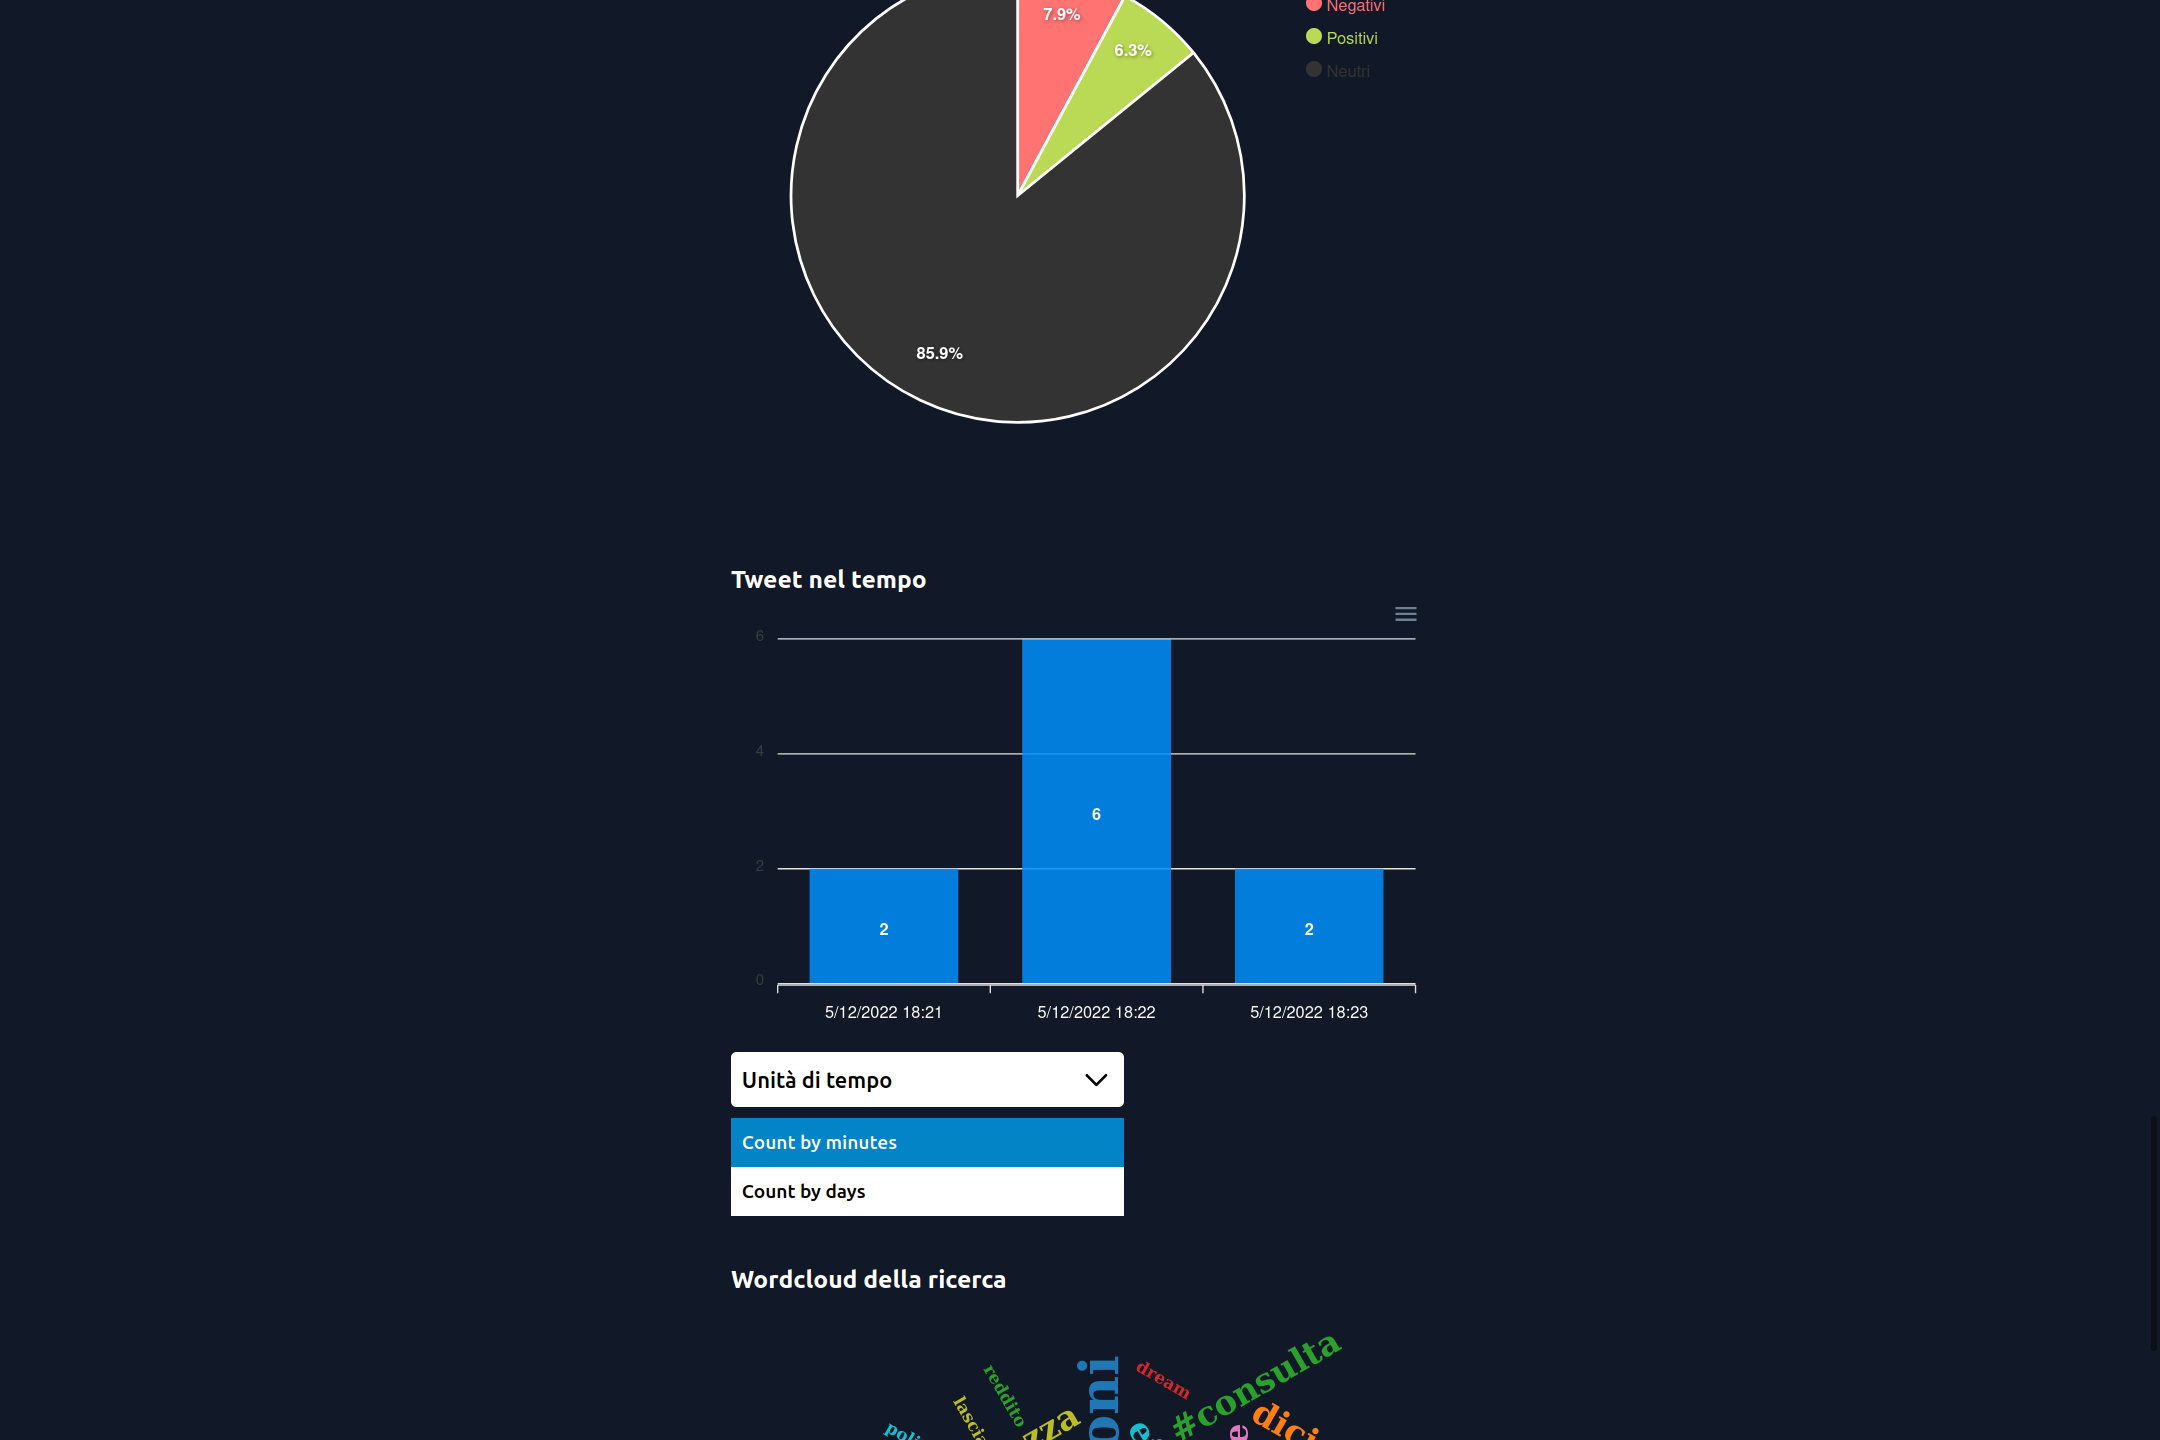
\includegraphics[scale=0.15]{reviews/sprint_review1205.png}
    \label{fig:review3}
\end{figure}
\end{frame}
\begin{frame}{Sprint 3, 16 Novembre - 30 Novembre}
\framesubtitle{Pratiche di CI, CD}
Abbiamo deciso fin da subito di creare una pipeline per l'automatizzazione dei test, build e del deploy sulle macchine di dipartimento.
\begin{figure}[H]
    \centering
    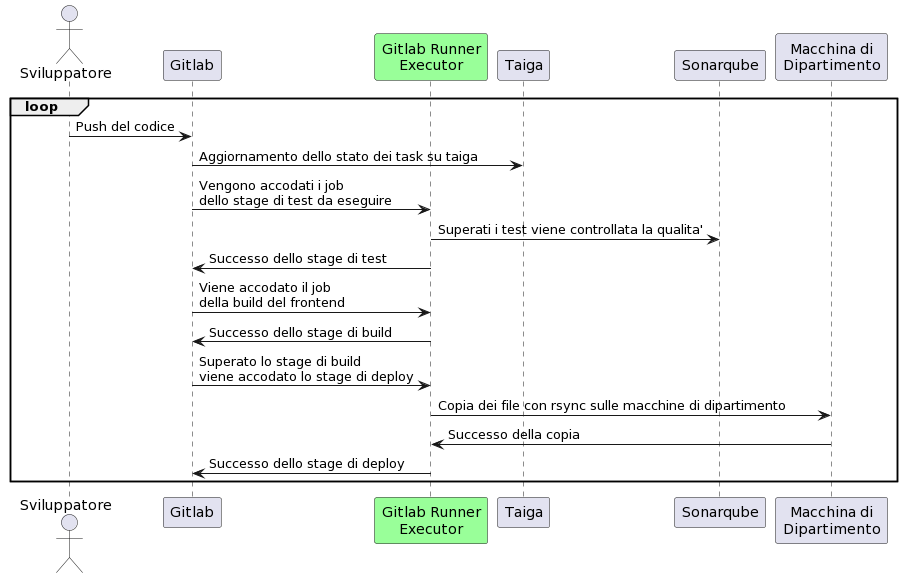
\includegraphics[scale=0.18]{misc/cicd.png}
    \caption{Diagramma di sequenza, creato con plantuml}
    \label{fig:pipeline}
\end{figure}
\end{frame}
\begin{frame}{Sprint 3, 16 Novembre - 30 Novembre}
\framesubtitle{\href{https://taiga.hjkl.gq/project/ingsw2022-team3/wiki/retrospettiva-sprint-3}{Retrospettiva}}
Anche se non siamo riusciti a completare tutte le US che ci eravamo imposti di completare, non \`e stato un grosso problema perch\'e eravamo a buon punto con tutte le funzionalit\'a da implementare.\\
Tra i punti su cui migliorare, per lo sprint 4 abbiamo pensato alla situazione dei test del frontend e del backend. \\
\href{https://taiga.hjkl.gq/project/ingsw2022-team3/wiki/retrospettiva-sprint-4}{Retrospettiva su taiga}
\end{frame}
\begin{frame}{Sprint 4, 30 Novembre - 14 Dicembre}
\framesubtitle{Sprint goal \& \href{https://taiga.hjkl.gq/project/ingsw2022-team3/taskboard/sprint-4-5}{backlog}}
Per questo sprint, poich\'e volevamo consegnare prima di Natale, ci siamo concentrati sul seguente goal: \\
Portare al professore un client che tra le altre funzionalit\'a gi\'a implementate, permettesse di giocare agli scacchi e ottenere interessanti info sul fantacitorio. \\
Backlog:
\begin{itemize}
    \item scacchi, raccolta delle mosse votate (23 punti)
    \item scacchi, mossa del giocatore (18 punti)
    \item fantacitorio, classifica dei politici (26 punti)
    \item fantacitorio, squadre di un utente (19 punti)
    \item fantacitorio, squadre della settimana (24 punti)
\end{itemize}
\end{frame}
\begin{frame}{Sprint 4, 30 Novembre - 14 Dicembre}
\framesubtitle{Lo sprint}
Questo \`e stato uno sprint impegnativo, siamo riusciti a chiudere lo sprint senza lasciare alcuna US aperta. \\
Inoltre ci siamo concentrati sull'aumentare la coverage, per riuscire a portare alla discussione finale una percentuale di almeno il 50\%.
\end{frame}
\begin{frame}{Sprint 4, 30 Novembre - 14 Dicembre}
\framesubtitle{\href{https://taiga.hjkl.gq/project/ingsw2022-team3/wiki/demo-finale}{Lo stato di avanzamento}}
\begin{figure}[H]
    \centering
    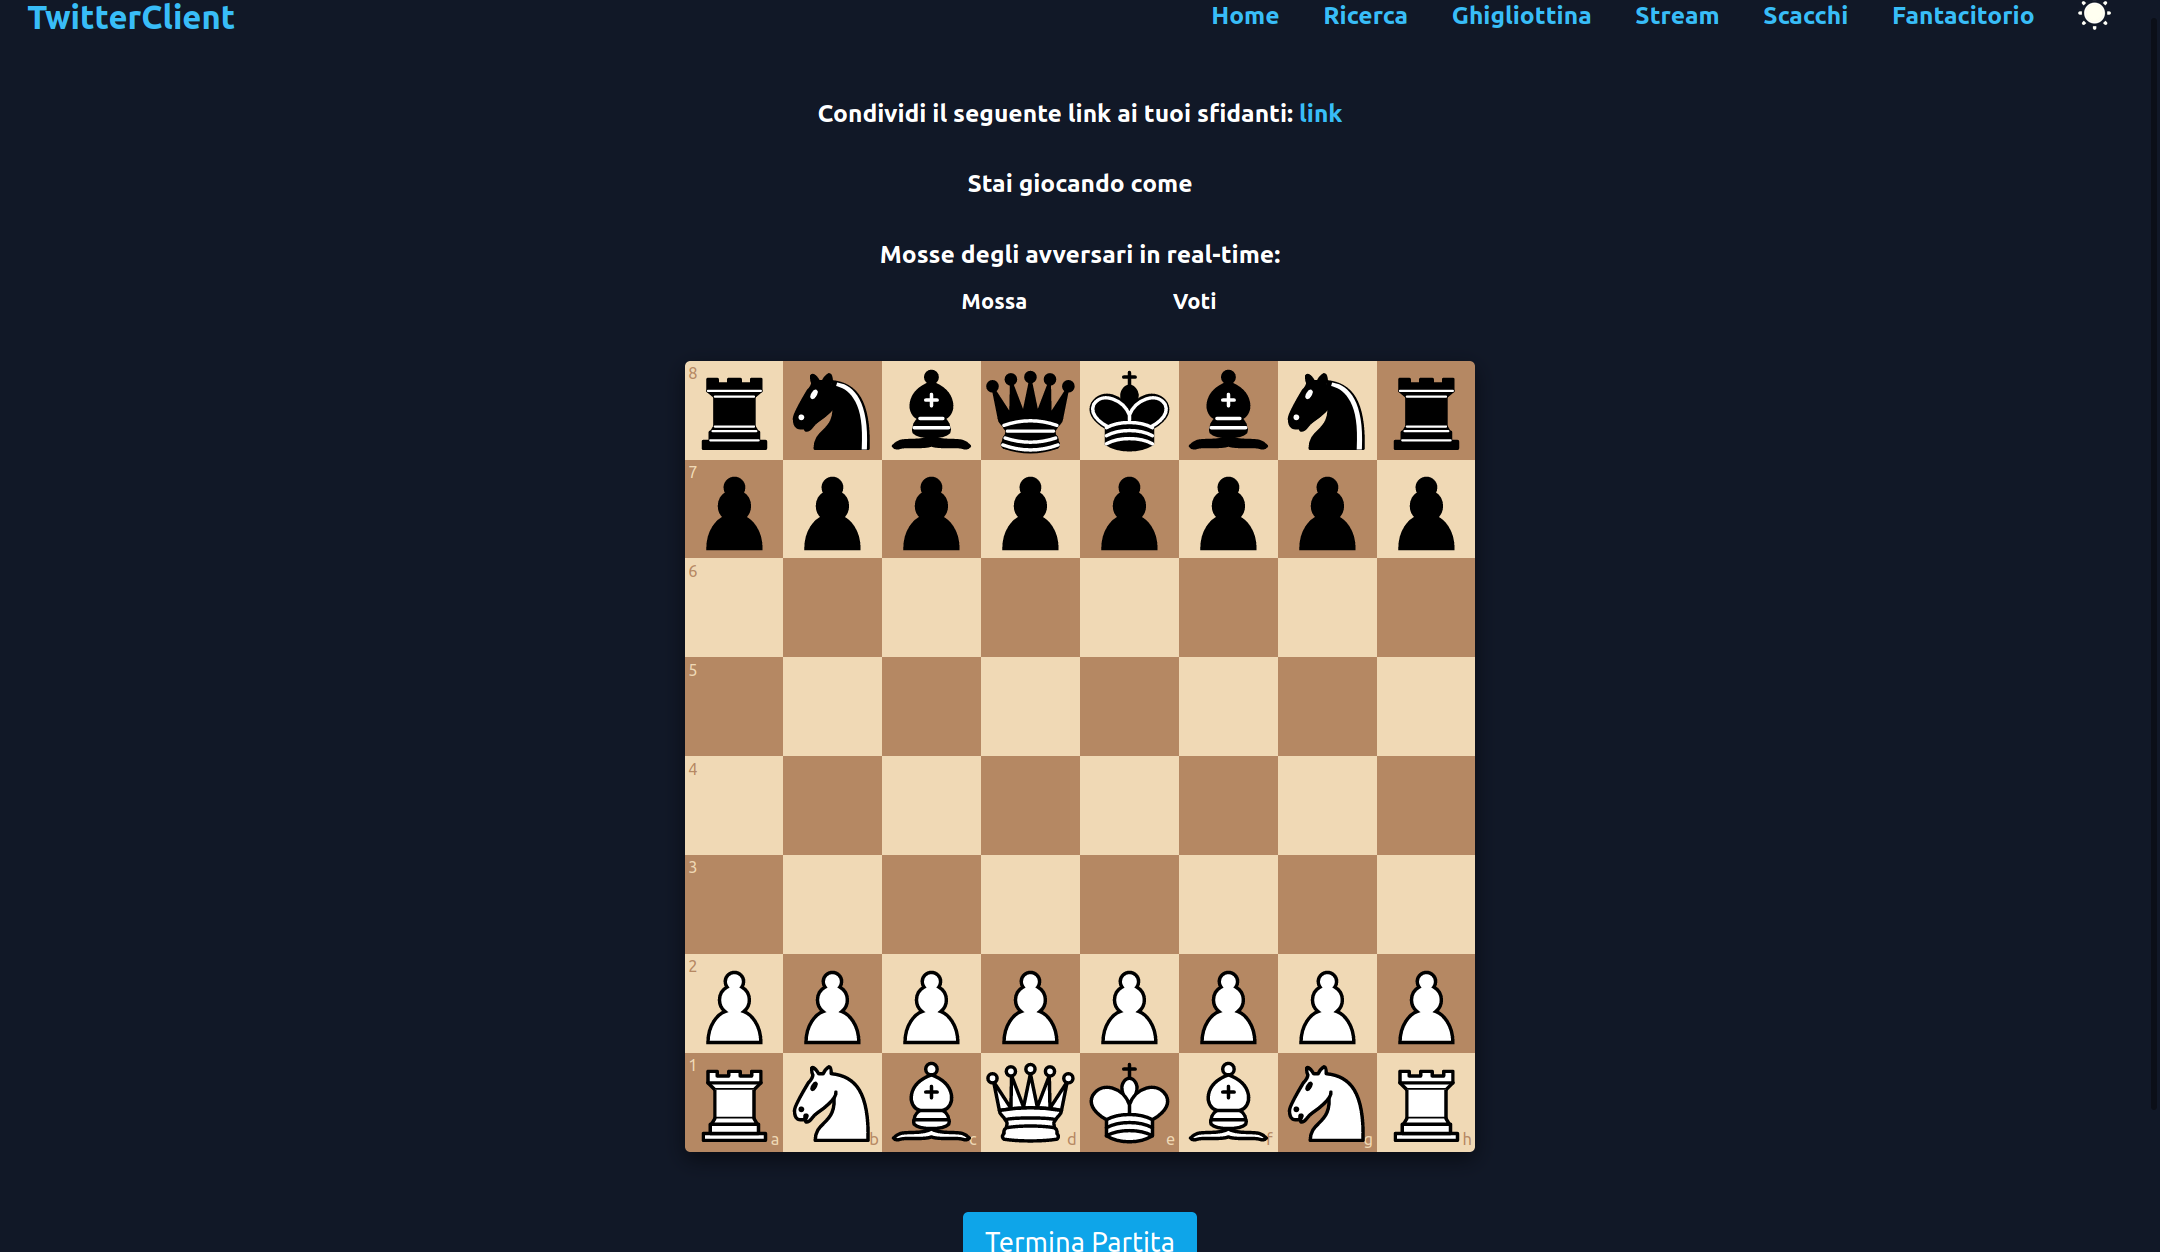
\includegraphics[scale=0.15]{reviews/scacchi_demo.png}
    \label{fig:scacchi}
\end{figure}
\end{frame}
\begin{frame}{Sprint 4, 30 Novembre - 14 Dicembre}
\framesubtitle{Retrospettiva}
Lo sprint \`e andato bene, siamo riusciti a completare lo sviluppo e raggiungere lo sprint goal. \\
Per\'o sono state riscontrate le seguenti criticit\'a: \\
\begin{itemize}
    \item La comunicazione, di alcuni componenti del team, \`e stata scarsa.
    \item La coverage del frontend, avremmo avuto bisogno di un altro sprint per riuscire a testare a fondo i nostri componenti.
\end{itemize}
\href{https://taiga.hjkl.gq/project/ingsw2022-team3/wiki/retrospettiva-sprint-4}{Retrospettiva su taiga}
\end{frame}
\begin{frame}{Conclusioni}
\framesubtitle{Gitinspector}
\begin{figure}[H]
    \centering
    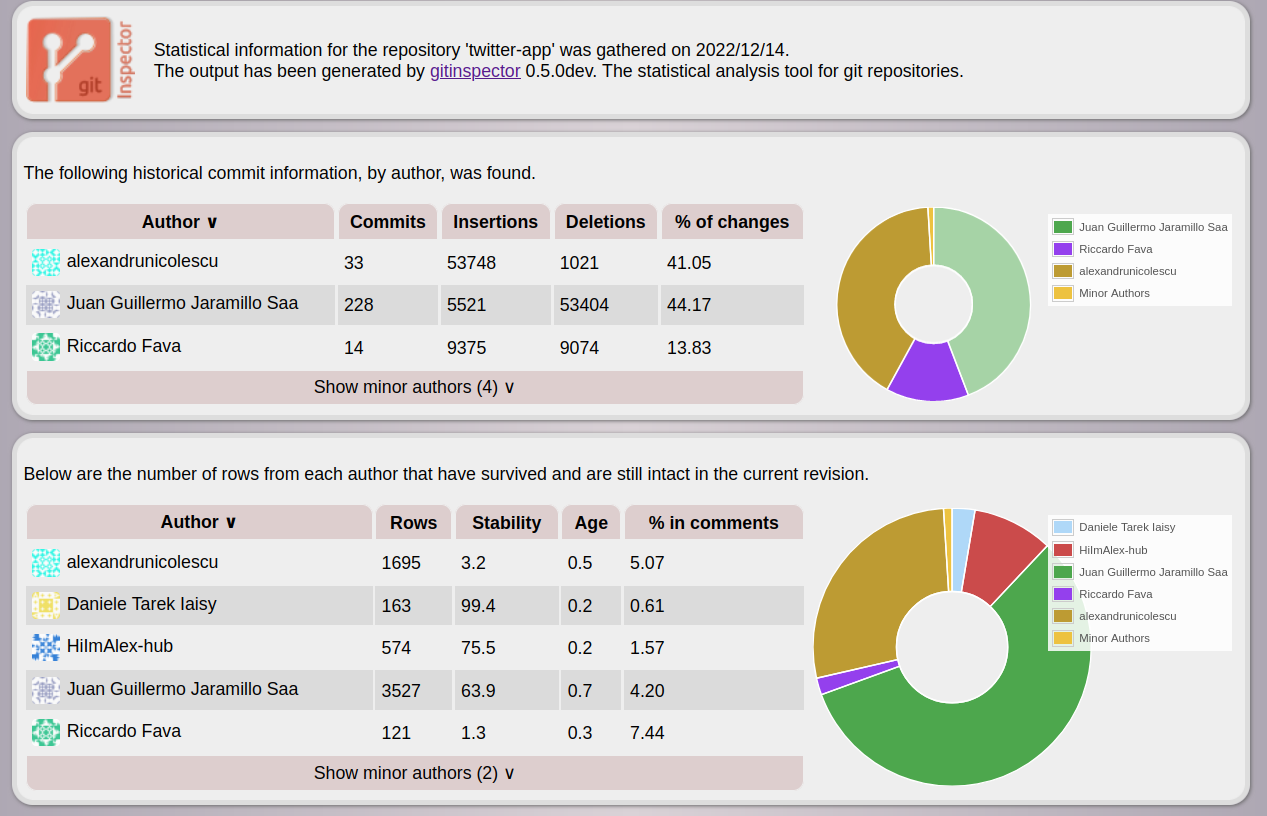
\includegraphics[scale=0.18]{misc/inspector_finale.png}
    \label{fig:inspector}
\end{figure}
\end{frame}
\begin{frame}{Conclusioni}
\framesubtitle{Qualit\'a}
\begin{figure}[H]
    \centering
    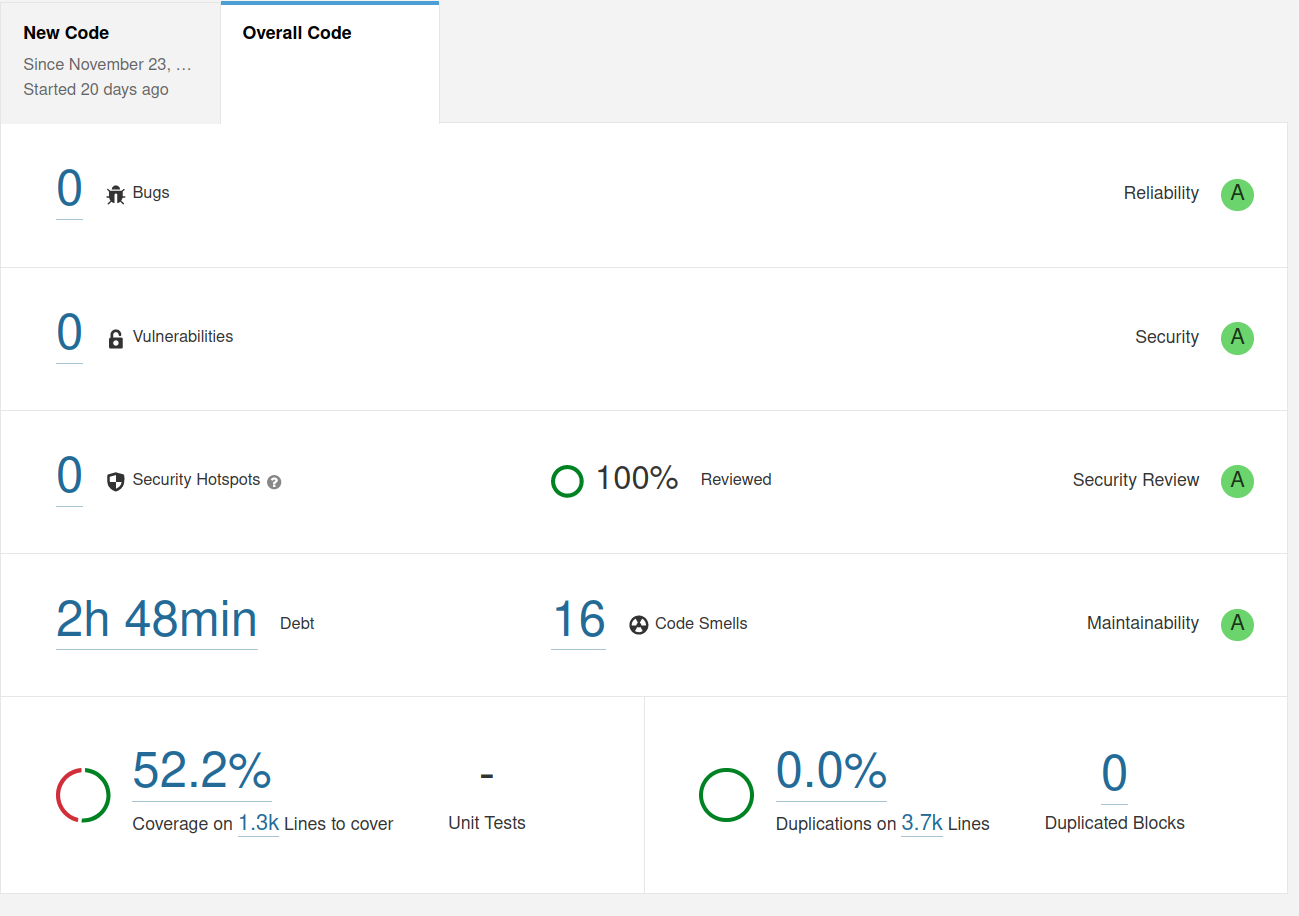
\includegraphics[scale=0.18]{misc/qube_analysis.png}
    \label{fig:qube}
\end{figure}
\end{frame}
\begin{frame}{Conclusioni}
\framesubtitle{Burndown complessivo}
\begin{figure}[H]
    \centering
    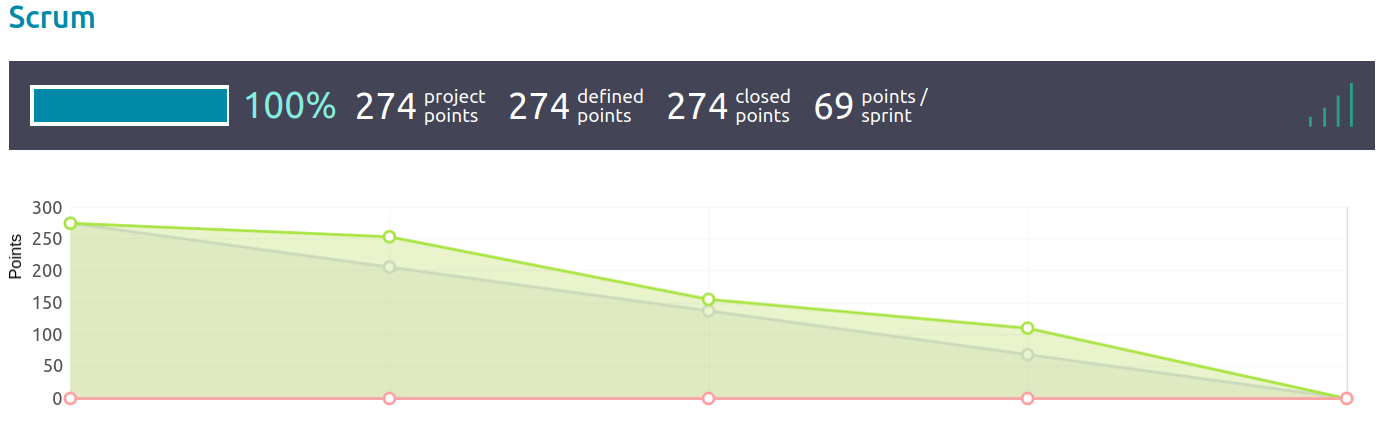
\includegraphics[scale=0.18]{misc/burndown_finale.png}
    \label{fig:finalburndown}
\end{figure}
\end{frame}
\begin{frame}{}
\centering
\usebeamerfont{frametitle}\usebeamercolor[fg]{frametitle}
Grazie per l'attenzione
\end{frame}
\end{document}
